

\documentclass{beamer}
\usepackage[super]{nth}

\usetheme{Madrid}

\makeatother
\setbeamertemplate{footline}
{
  \leavevmode%
  \hbox{%
  \begin{beamercolorbox}[wd=.2\paperwidth,ht=2.25ex,dp=1ex,center]{author in head/foot}%
    \usebeamerfont{author in head/foot}\insertshortauthor
  \end{beamercolorbox}%
  \begin{beamercolorbox}[wd=.8\paperwidth,ht=2.25ex,dp=1ex,center]{title in head/foot}%
    \usebeamerfont{title in head/foot}\insertshorttitle\hspace*{3em}
    \insertframenumber{} / \inserttotalframenumber\hspace*{1ex}
  \end{beamercolorbox}}%
  \vskip0pt%
}
\makeatletter
\setbeamertemplate{navigation symbols}{}
\title{PhD Application for The PhD Thesis\\ "Decentralized Fog Computing Infrastructure Control"}


\subtitle{}

\author{Ali J. Fahs}%\\ Supervisor: Professor Guillaume Pierre}



\institute[Institut de Recherche en Informatique et Systèmes Aléatoires (IRISA)] % (optional, but mostly needed)
{
 Supervised by Professor Guillaume Pierre 
   }

\date{Audition, \nth{8} of June, 2017}

\subject{PhD Application}

\begin{document}

\begin{frame}
  \titlepage
\end{frame}

\begin{frame}{Outline}
  \tableofcontents
 
\end{frame}

%%%%%%%%%%%%%%%%%%%%%%%%%%%%%%%%%%%%%%%
\section{Personal Presentation}
\begin{frame}{Personal Presentation}
\begin{itemize}
\item A double diploma student.
\begin{itemize}
\item Engineering diploma in telecommunication and computer science - \textbf{Lebanese University, Faculty of engineering (ULFG)}.
\item Master's degree in Informatics Grenoble (MoSIG) Parallel, Distributed Systems Track - \textbf{Grenoble INP} (Institut national polytechnique), \textbf{Ensimag} (\'Ecole nationale sup\'erieure d'informatique et de math\'ematiques appliqu\'ees de Grenoble) jointly with \textbf{UGA} (universit\'e grenoble alpes), \textbf{IMAG} (Informatique, math\'ematiques, math\'ematiques appliqu\'ees de Grenoble).
\end{itemize}

\item Research interest: \alert{Distributed systems, Networking.}
\item Master's thesis "Distributed Approach for Cross-Layer Resource Allocation in Wireless Sensor Networks" Jointly between LIG (Laboratoire d'Informatique de Grenoble) and VERIMAG.
\end{itemize}

 
\end{frame}


%%%%%%%%%%%%%%%%%%%%%%%%%%%%%%%%%%%%%%%%%%%%%%%%%%%%%
\section{Master Thesis}

\begin{frame}{Master Thesis}

\begin{minipage}[t]{0.48\linewidth}

\begin{block}{Overview}
    \begin{itemize}
    \item IEEE802.15.4: Wireless sensor network standard. 
    \item<2-> Time-slotted channel hopping (TSCH), The Medium access layer control.  
     \item<3-> 6TiSCH: IPv6 over IEEE802.15.4e TSCH. 
     \end{itemize}
    \end{block}
\end{minipage}\hfill
\begin{minipage}[t]{0.48\linewidth}
\centering
\begin{figure}[p]

\item<2-> 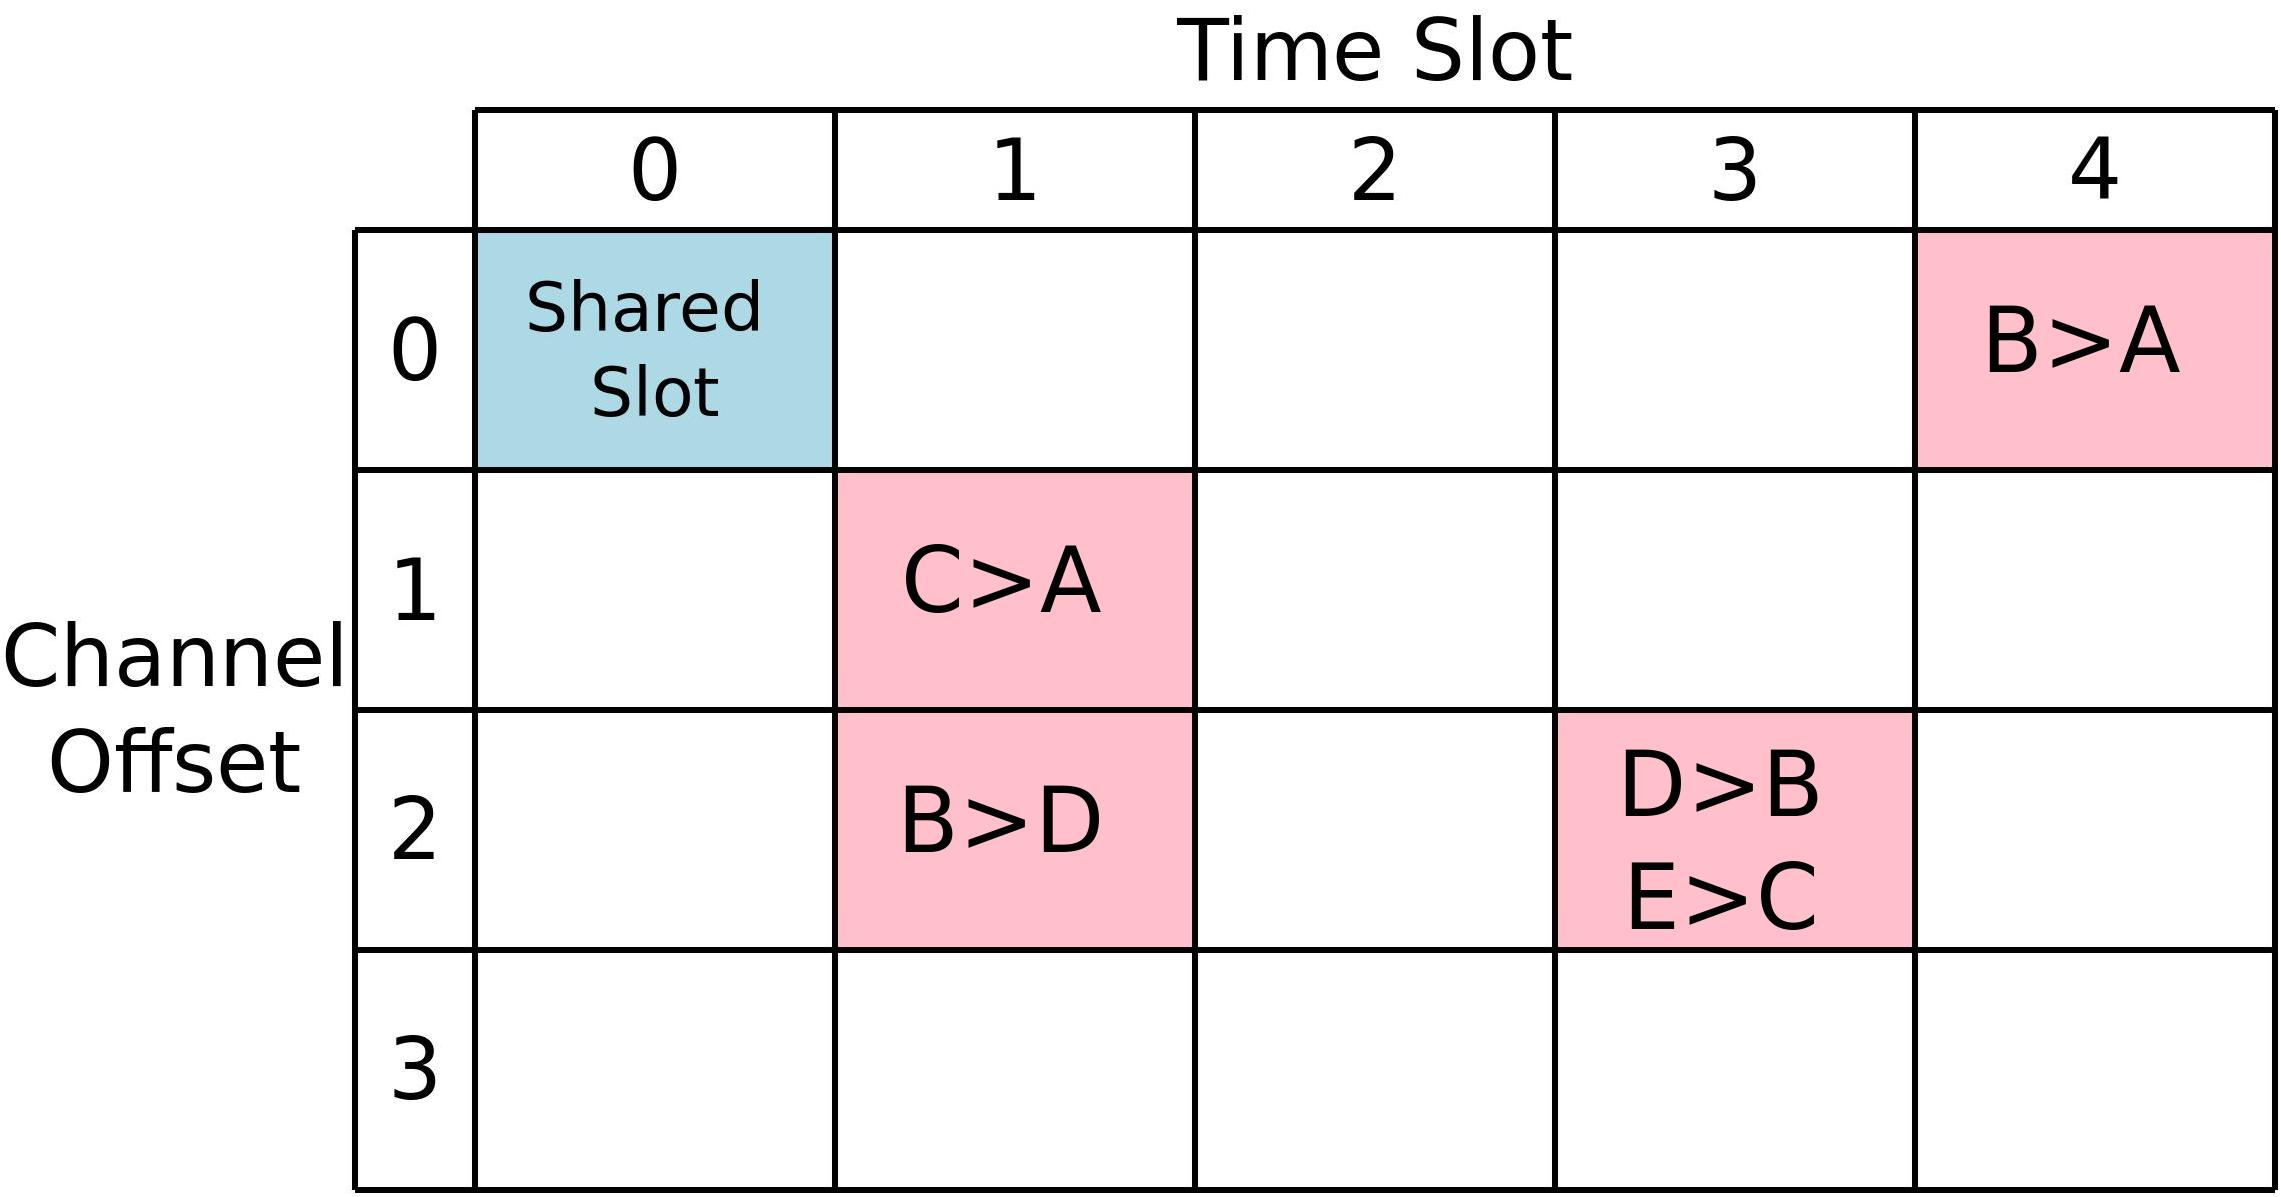
\includegraphics[width=\linewidth]{TSCH.jpeg}

\end{figure}

\end{minipage}
\end{frame}



\begin{frame}{Master Thesis}

\begin{minipage}[t]{0.48\linewidth}

\begin{block}{Challenges}
    \begin{itemize}
    
   
    \item High collision rates in TSCH dedicated cells.
     \item<2-> Cause: no coordination between nodes. 
      \item<3-> Lack of central entity. 
      
     
    
    \end{itemize}
    \end{block}
\end{minipage}\hfill
\begin{minipage}[t]{0.48\linewidth}
\centering
\begin{figure}[p]

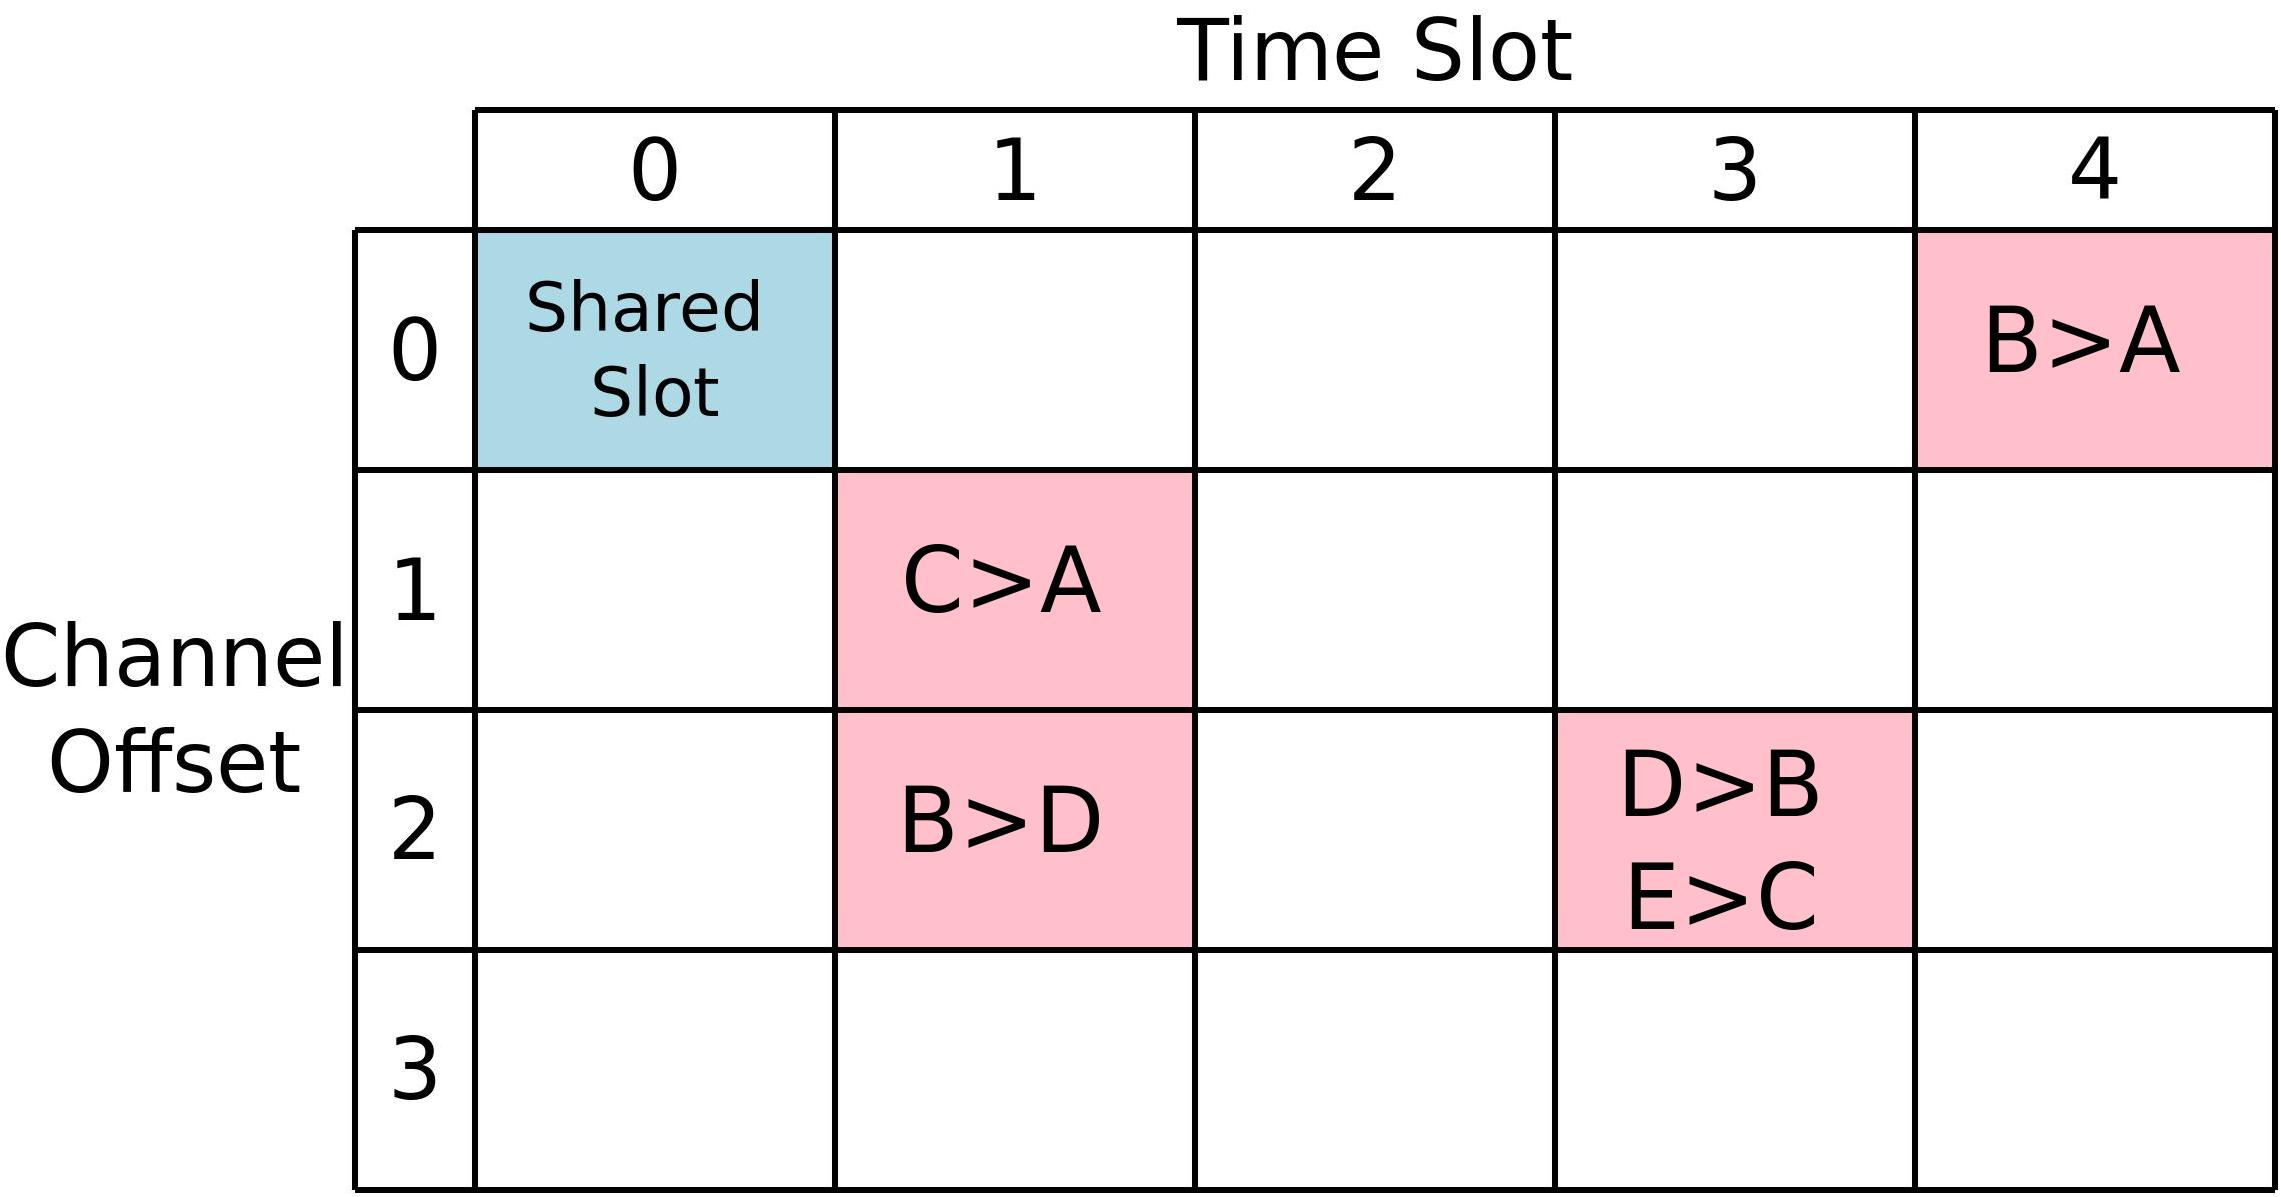
\includegraphics[width=\linewidth]{TSCH.jpeg}

\end{figure}
\begin{figure}[p]


\item<2-> 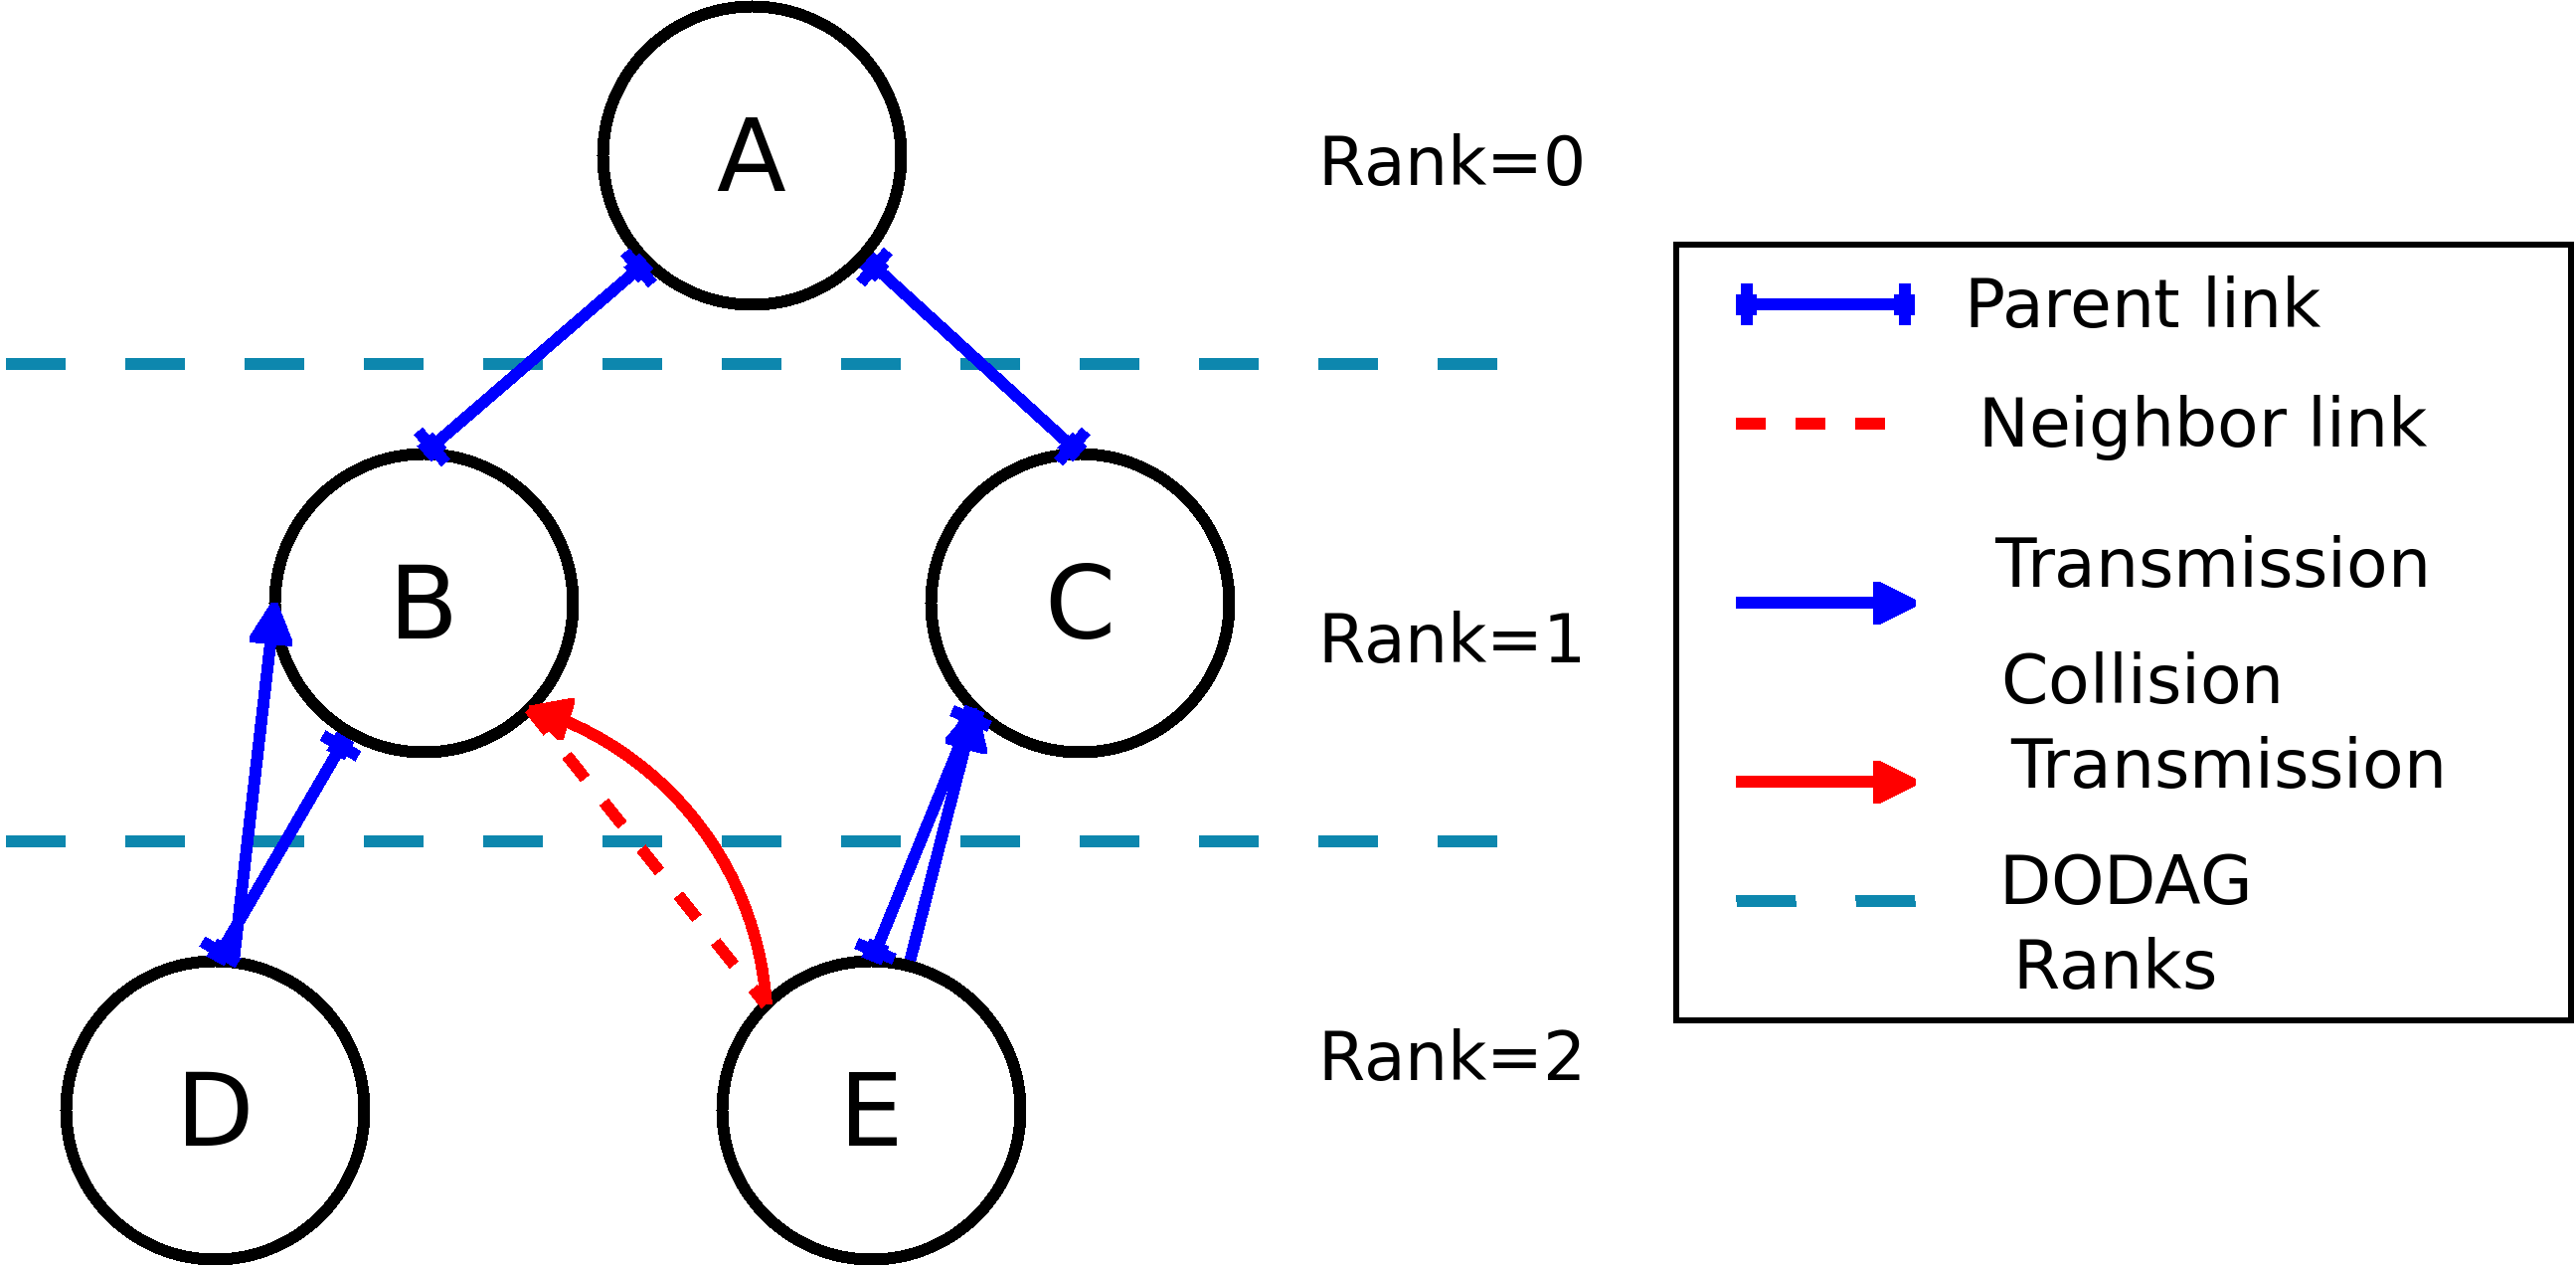
\includegraphics[width=\linewidth]{Diagram1.png}
\end{figure}
\end{minipage}
\end{frame}

\begin{frame}{Master Thesis}

\begin{block}{Proposed Mechanism}
    \begin{itemize}
    \item Local mutual exclusion: every node passively learn the schedule of their neighbors. 
    \item<2-> Entirely local algorithm, no new messages were introduced.
     \item<3-> Result: 70\% reduction in the colliding Tx cells.
     
    \end{itemize}
    \end{block}


\centering
\begin{figure}[ht]

\item<2-> 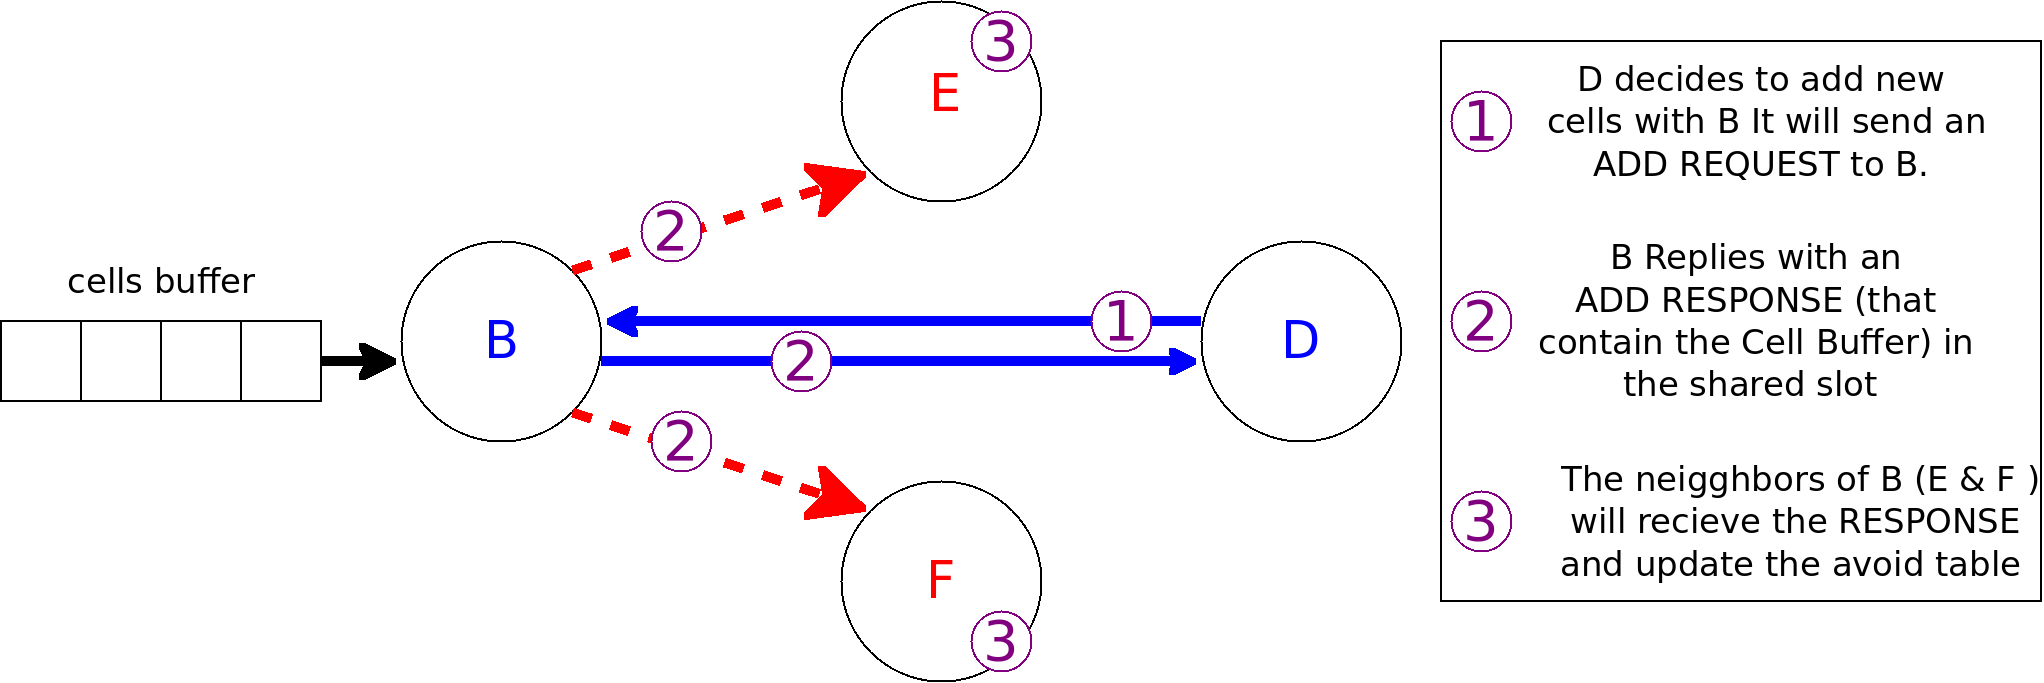
\includegraphics[width=.85\linewidth]{collision.png}

\end{figure}
\end{frame}

\begin{frame}{Master thesis Results}


\begin{figure}[ht]


 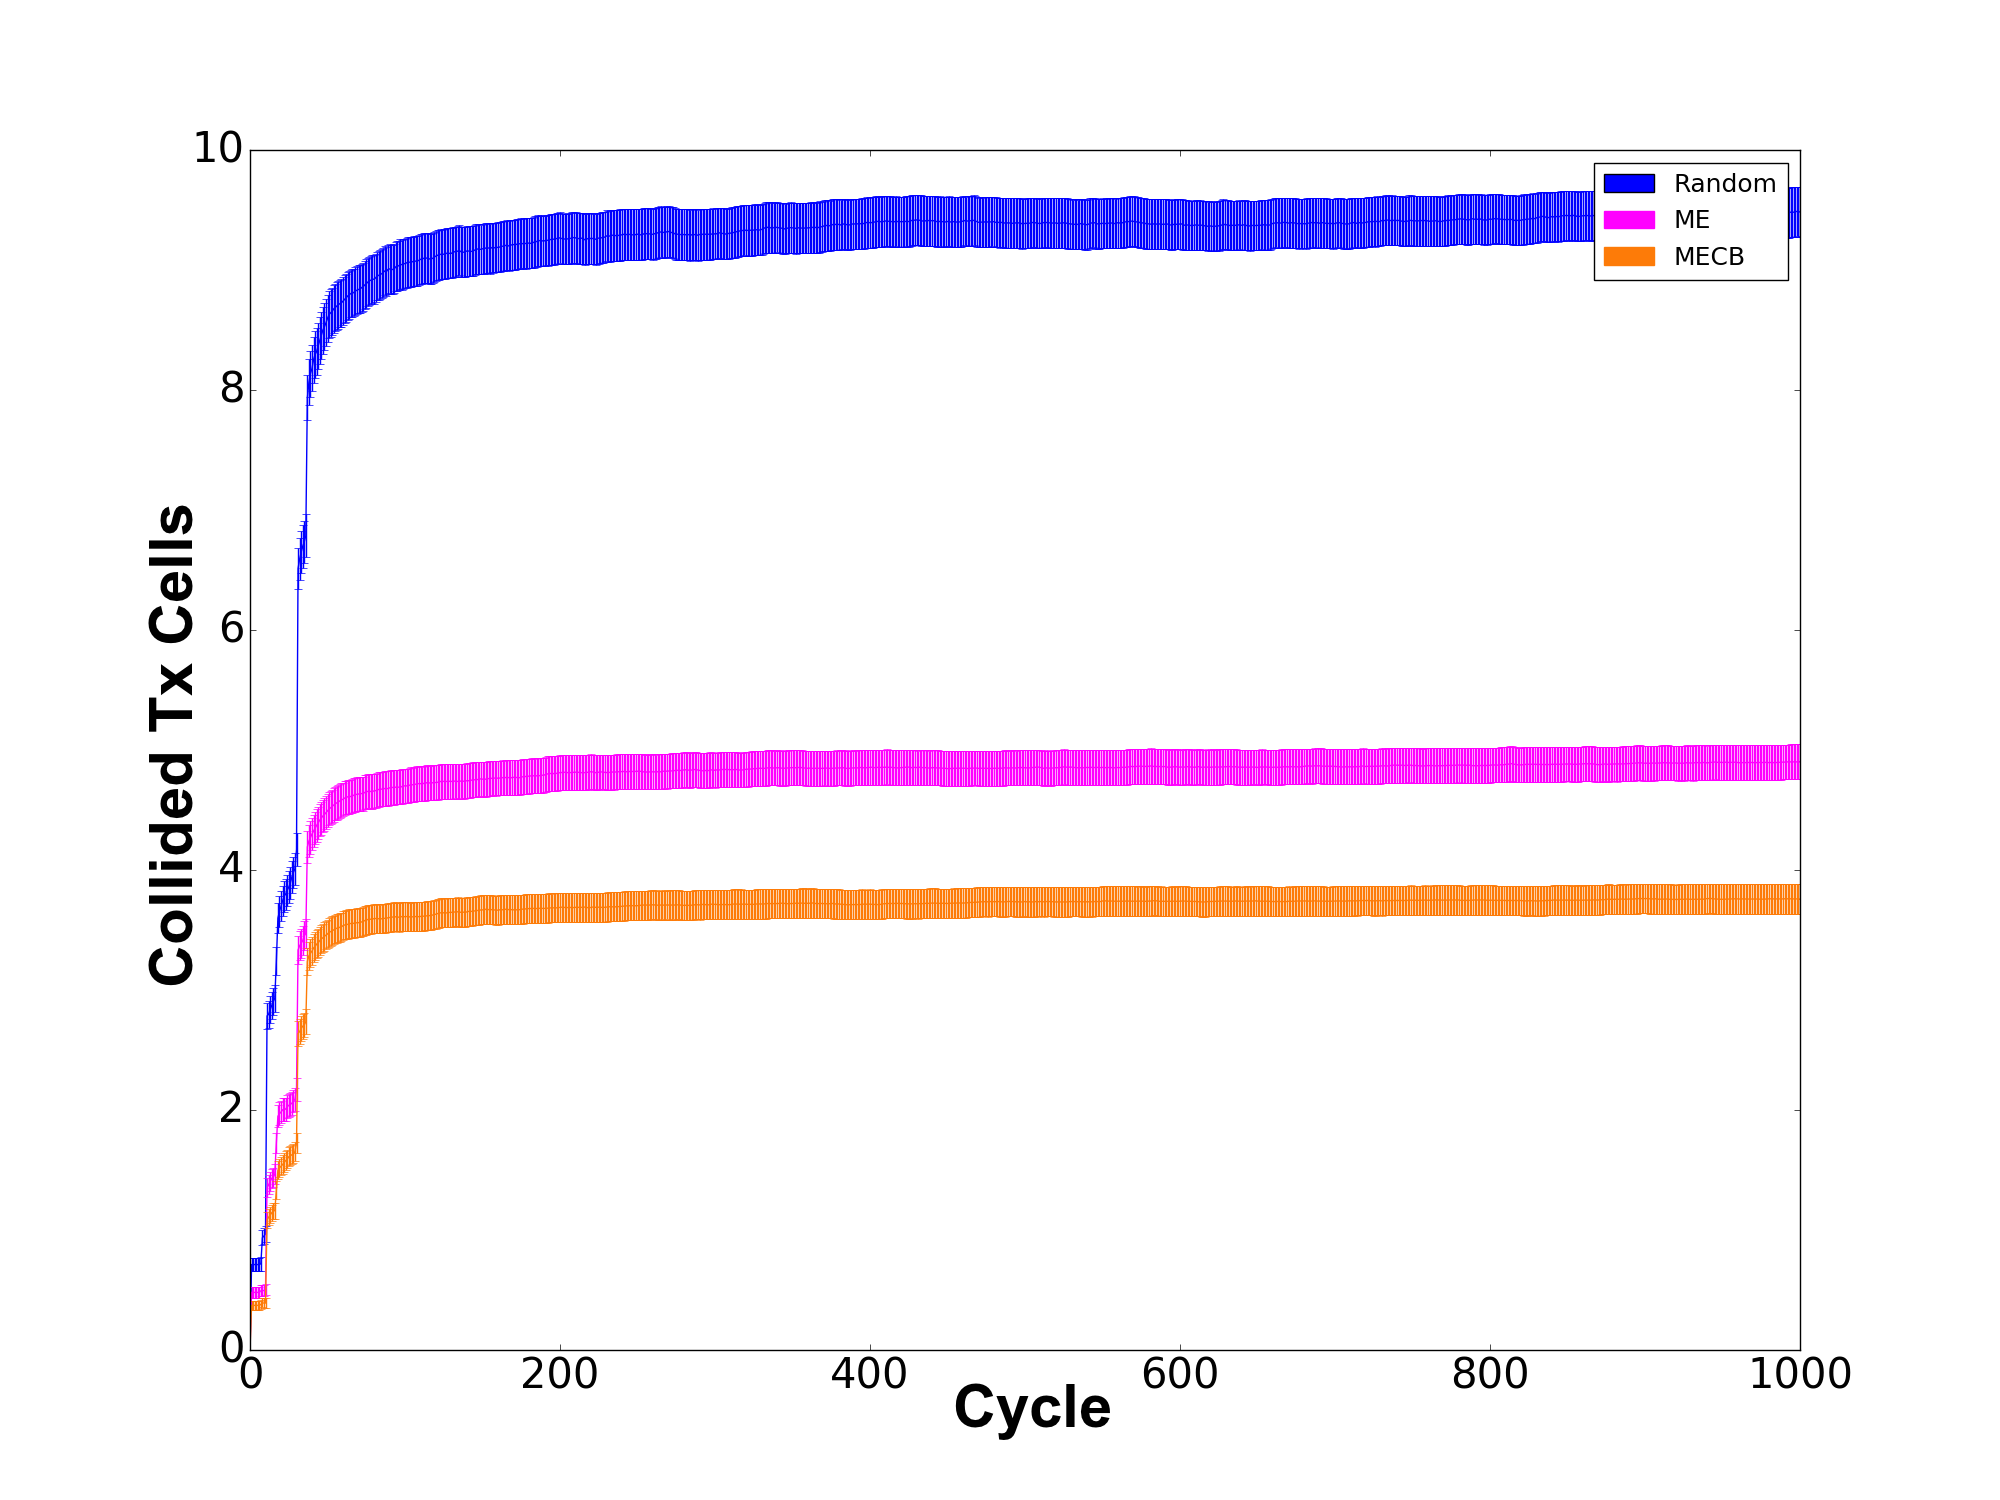
\includegraphics[width=.78\linewidth]{Graph2.png}
\end{figure}


\begin{itemize}
\item Paper to be submitted to conference \textbf{WiMob 2017}.
\end{itemize}
\end{frame}


%%%%%%%%%%%%%%%%%%%%%%%%%%%%%%%%%%%%%%%%%%%%%%%%%%%%%
\section{State-of-the-Art for Edge Clouding}

\begin{frame}{State-of-the-Art for Edge Clouding}

\begin{block}{Cloud Infrastructure}
    \begin{itemize}
    \item  Pros: extremely flexible and powerful.
    \item<2->  Cons: Clouding disadvantages: latency, mobility, {\em etc}...

    \end{itemize}
    \end{block}

\end{frame}

\begin{frame}{State-of-the-Art for Edge Clouding}

\begin{block}{Cloud Infrastructure}
    \begin{itemize}
    \item  Pros: extremely flexible and powerful.
    \item  Cons: Clouding disadvantages: latency, mobility, {\em etc}...

    \end{itemize}
    \end{block}

\begin{block}{Edge clouds}
    \begin{itemize}
    \item Idea: deploying cloud applications in the immediate end user proximity.
    \item<2-> Results: better end to end latency and application interactivity, less long-distance traffic.
     \item<3-> Infrastructure based on single-board computers: small, cheap, can  be deployed everywhere.
   
    \end{itemize}
    \end{block}
 {\tiny *references: 1-Yi, Shanhe, Cheng Li, and Qun Li. "A survey of fog computing: concepts, applications and issues." Proceedings of the 2015 Workshop on Mobile Big Data. ACM, 2015.\\
2- Van Kempen, Alexandre, et al. "MEC-ConPaaS: An experimental single-board based mobile edge cloud." IEEE Mobile Cloud Conference. 2017.}

\end{frame}

\section{PhD Topic}
\begin{frame}{PhD Topic}
 \begin{block}{Challenges of Fog Computing}
    \begin{itemize}
    \item Infrastructure based on very large numbers of unreliable and distributed servers.
    \item<2-> But the control remains centralized.
    \item<3-> Drawbacks: unnecessary traffic, latency, robustness
    \item<4-> Application developers should not handle the complexity of application deployment, fault tolerance, reconfiguration, or elasticity.
      
    \end{itemize}
    
    \end{block}
    
    \begin{figure}[ht]


 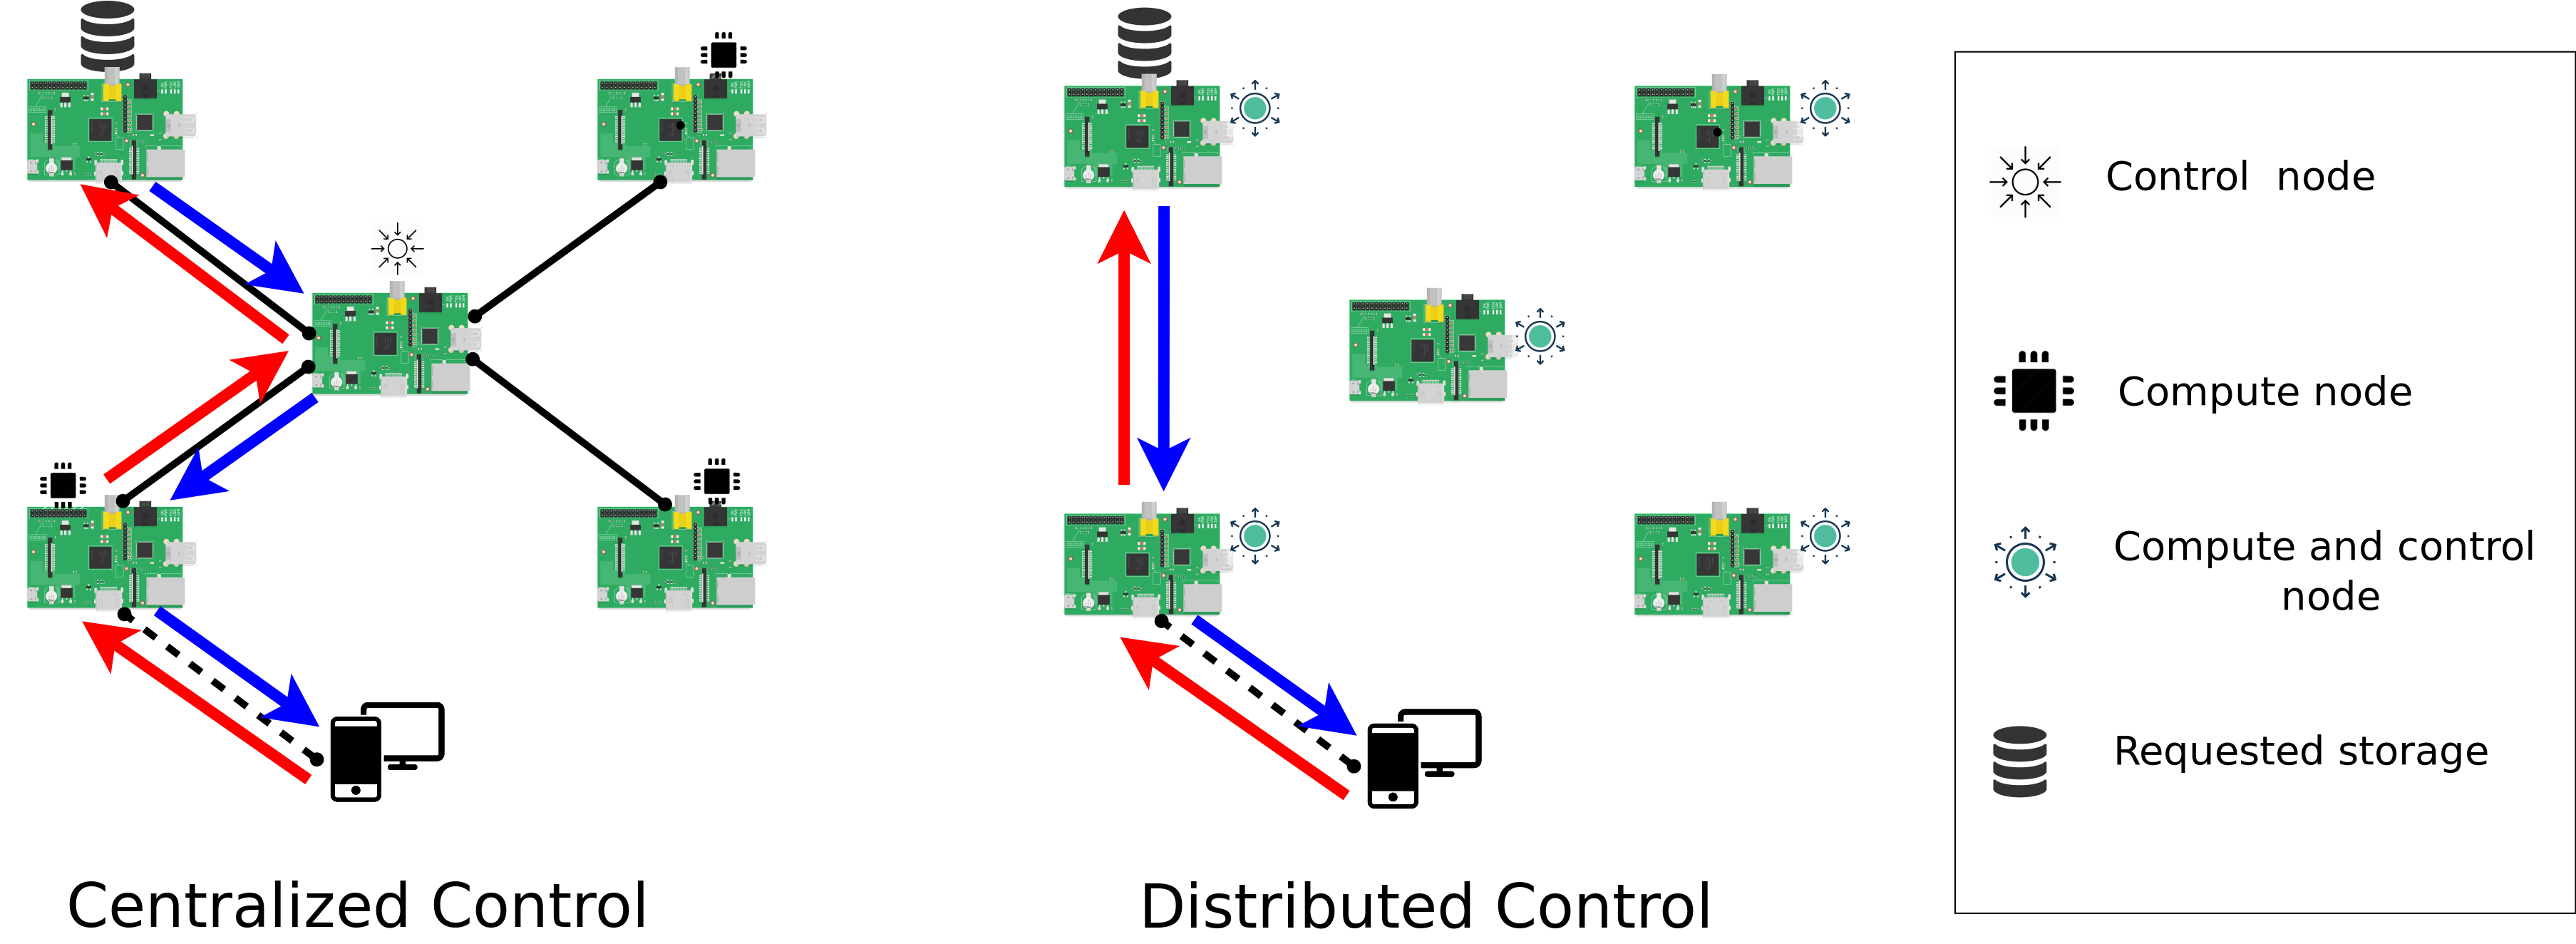
\includegraphics[width=.85\linewidth]{fog.png}
\end{figure}
\end{frame}

\begin{frame}{PhD Topic}


\begin{block}{Objectives}
    \begin{itemize}
    
    \item Designing fully distributed control mechanisms: every compute node is also a control node. 
    \item<2->  Compare to centralized alternatives. 
    \item<3->  One interesting direction: gossip-based algorithms for the coordination of multiple schedulers.
      
    \end{itemize}
    
    \end{block}
 {\tiny *references: Jelasity, Márk, et al. "Gossip-based peer sampling." ACM Transactions on Computer Systems (TOCS) 25.3 (2007).}    
    
 \end{frame}
    
  
    

 

\section{Project Perspective}
\begin{frame}{Perspective}

\begin{block}{Project Perspective}
    \begin{itemize}
    
    \item  Edge clouds are very new $ \implies $ opportunities for impact
    \item<2-> An H2020 project coordinated by Prof. Pierre will start soon on fog computing.
    
      
    \end{itemize}
    
    \end{block}

\begin{block}{Personal Perspective}
    \begin{itemize}
    
    \item<3-> Spend 3 years of my life with a subject that I'm completely interested in, so I can reach my max potential.
    
    \item<4-> The field of cloud and distributed systems is currently undergoing a revolution, and I want to be a part of this revolution.
   
   
    
    \end{itemize}
    
    \end{block}
   
    


\end{frame}


\section*{last}

\begin{frame}
\begin{tabular}{ccc}

\includegraphics[page=10, width=0.3\textwidth]{ali.pdf} &

\includegraphics[page=15, width=0.3\textwidth]{ali.pdf} &

\includegraphics[page=16, width=0.3\textwidth]{ali.pdf} \\


\includegraphics[page=22, width=0.3\textwidth]{ali.pdf} &

\includegraphics[page=26, width=0.3\textwidth]{ali.pdf} &

\includegraphics[page=30, width=0.3\textwidth]{ali.pdf} \\




\end{tabular}

\begin{block}{}
\centering Thanks for your attention!\\
Questions?
\end{block}
\end{frame}










\end{document}


